\documentclass[10pt,a4paper]{article}
\usepackage[T1]{fontenc}
\usepackage[utf8]{inputenc}
\usepackage{lmodern}
\usepackage[a4paper,left=38mm,right=38mm,top=34mm,bottom=38mm]{geometry}
\usepackage{amsmath,amssymb}
\usepackage{xcolor}
\usepackage{tikz}
\usetikzlibrary{arrows.meta,patterns}
\usepackage{float}
\usepackage[font=small,labelfont=bf,skip=6pt]{caption}
\usepackage{booktabs}
\usepackage{enumitem}
\usepackage[hidelinks]{hyperref}
\setlength{\parindent}{0pt}
\setlength{\parskip}{0.55em}
\setlength{\textfloatsep}{14pt}
\setlength{\intextsep}{14pt}

\definecolor{ink}{HTML}{1D2733}
\definecolor{inksoft}{HTML}{55606C}
\definecolor{gridc}{HTML}{BCC2BA}
\definecolor{chosen}{HTML}{24525F}
\definecolor{blockedc}{HTML}{C9CEC7}
\definecolor{hatch}{HTML}{8F978E}
\definecolor{candc}{HTML}{C27A12}
\definecolor{candtint}{HTML}{F6DFB6}
\definecolor{cand2c}{HTML}{6D55B3}
\definecolor{cand2tint}{HTML}{DDD5F3}
\definecolor{focus}{HTML}{2C7DA0}
\definecolor{focustint}{HTML}{CFE6EF}
\definecolor{bad}{HTML}{C0392B}
\definecolor{okc}{HTML}{3F7D4A}

\newcommand{\incode}{\textsf{\scriptsize\color{okc}[in code]}}
\newcommand{\proposed}{\textsf{\scriptsize\color{candc}[proposed]}}
\newcommand{\onmap}{\par\medskip\textsf{\small\bfseries\color{inksoft}On the map}\par}
\newcommand{\interms}{\par\medskip\textsf{\small\bfseries\color{inksoft}In .conditions}\par}
\newcommand{\code}[1]{\texttt{#1}}
\newcommand{\T}[1]{\ensuremath{\{#1\}}}
\newenvironment{algebra}{\begin{center}\begin{minipage}{0.92\linewidth}\small\setlength{\parskip}{0.2em}}{\end{minipage}\end{center}}
\newcommand{\cmt}[1]{{\color{inksoft}\textit{#1}}}


\title{\textsf{Unblocking}\\[0.3em]\large the rule as implemented, against suspending and against unblocking inside the pass}
\date{16 November 2026}
\author{}

\begin{document}
\maketitle
\thispagestyle{empty}

A candidate $Z$ is \emph{refuted} when choosing it would force two cells that block each other: two diagonal neighbours, both to be chosen. This note describes what the algorithm now does with such a candidate, why that is sound, and how it compares with the two earlier approaches: suspending $Z$ for a pass (until 15 November), and unblocking inside the pass (15 to 16 November). Section numbers of the form ``F\,9'' refer to \emph{Conditions and the Map} (\code{docs/foundation}).

%------------------------------------------------------------------
\section{The situation}

\begin{figure}[H]\centering
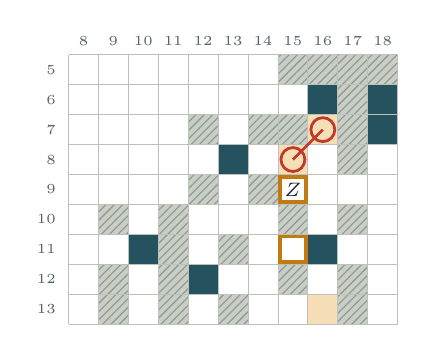
\begin{tikzpicture}[x=0.38cm,y=0.38cm,baseline=(current bounding box.north)]
\node[font=\tiny,text=inksoft] at (0.5,0.45) {8};
\node[font=\tiny,text=inksoft] at (1.5,0.45) {9};
\node[font=\tiny,text=inksoft] at (2.5,0.45) {10};
\node[font=\tiny,text=inksoft] at (3.5,0.45) {11};
\node[font=\tiny,text=inksoft] at (4.5,0.45) {12};
\node[font=\tiny,text=inksoft] at (5.5,0.45) {13};
\node[font=\tiny,text=inksoft] at (6.5,0.45) {14};
\node[font=\tiny,text=inksoft] at (7.5,0.45) {15};
\node[font=\tiny,text=inksoft] at (8.5,0.45) {16};
\node[font=\tiny,text=inksoft] at (9.5,0.45) {17};
\node[font=\tiny,text=inksoft] at (10.5,0.45) {18};
\node[font=\tiny,text=inksoft,anchor=east] at (-0.1,-0.5) {5};
\node[font=\tiny,text=inksoft,anchor=east] at (-0.1,-1.5) {6};
\node[font=\tiny,text=inksoft,anchor=east] at (-0.1,-2.5) {7};
\node[font=\tiny,text=inksoft,anchor=east] at (-0.1,-3.5) {8};
\node[font=\tiny,text=inksoft,anchor=east] at (-0.1,-4.5) {9};
\node[font=\tiny,text=inksoft,anchor=east] at (-0.1,-5.5) {10};
\node[font=\tiny,text=inksoft,anchor=east] at (-0.1,-6.5) {11};
\node[font=\tiny,text=inksoft,anchor=east] at (-0.1,-7.5) {12};
\node[font=\tiny,text=inksoft,anchor=east] at (-0.1,-8.5) {13};
\fill[blockedc] (7,0) rectangle (8,-1);
\fill[pattern=north east lines,pattern color=hatch] (7,0) rectangle (8,-1);
\fill[blockedc] (8,0) rectangle (9,-1);
\fill[pattern=north east lines,pattern color=hatch] (8,0) rectangle (9,-1);
\fill[blockedc] (9,0) rectangle (10,-1);
\fill[pattern=north east lines,pattern color=hatch] (9,0) rectangle (10,-1);
\fill[blockedc] (10,0) rectangle (11,-1);
\fill[pattern=north east lines,pattern color=hatch] (10,0) rectangle (11,-1);
\fill[chosen] (8,-1) rectangle (9,-2);
\fill[blockedc] (9,-1) rectangle (10,-2);
\fill[pattern=north east lines,pattern color=hatch] (9,-1) rectangle (10,-2);
\fill[chosen] (10,-1) rectangle (11,-2);
\fill[blockedc] (4,-2) rectangle (5,-3);
\fill[pattern=north east lines,pattern color=hatch] (4,-2) rectangle (5,-3);
\fill[blockedc] (6,-2) rectangle (7,-3);
\fill[pattern=north east lines,pattern color=hatch] (6,-2) rectangle (7,-3);
\fill[blockedc] (7,-2) rectangle (8,-3);
\fill[pattern=north east lines,pattern color=hatch] (7,-2) rectangle (8,-3);
\fill[candtint] (8,-2) rectangle (9,-3);
\fill[blockedc] (9,-2) rectangle (10,-3);
\fill[pattern=north east lines,pattern color=hatch] (9,-2) rectangle (10,-3);
\fill[chosen] (10,-2) rectangle (11,-3);
\fill[chosen] (5,-3) rectangle (6,-4);
\fill[candtint] (7,-3) rectangle (8,-4);
\fill[blockedc] (9,-3) rectangle (10,-4);
\fill[pattern=north east lines,pattern color=hatch] (9,-3) rectangle (10,-4);
\fill[blockedc] (4,-4) rectangle (5,-5);
\fill[pattern=north east lines,pattern color=hatch] (4,-4) rectangle (5,-5);
\fill[blockedc] (6,-4) rectangle (7,-5);
\fill[pattern=north east lines,pattern color=hatch] (6,-4) rectangle (7,-5);
\fill[blockedc] (1,-5) rectangle (2,-6);
\fill[pattern=north east lines,pattern color=hatch] (1,-5) rectangle (2,-6);
\fill[blockedc] (3,-5) rectangle (4,-6);
\fill[pattern=north east lines,pattern color=hatch] (3,-5) rectangle (4,-6);
\fill[blockedc] (7,-5) rectangle (8,-6);
\fill[pattern=north east lines,pattern color=hatch] (7,-5) rectangle (8,-6);
\fill[blockedc] (9,-5) rectangle (10,-6);
\fill[pattern=north east lines,pattern color=hatch] (9,-5) rectangle (10,-6);
\fill[chosen] (2,-6) rectangle (3,-7);
\fill[blockedc] (3,-6) rectangle (4,-7);
\fill[pattern=north east lines,pattern color=hatch] (3,-6) rectangle (4,-7);
\fill[blockedc] (5,-6) rectangle (6,-7);
\fill[pattern=north east lines,pattern color=hatch] (5,-6) rectangle (6,-7);
\fill[chosen] (8,-6) rectangle (9,-7);
\fill[blockedc] (1,-7) rectangle (2,-8);
\fill[pattern=north east lines,pattern color=hatch] (1,-7) rectangle (2,-8);
\fill[blockedc] (3,-7) rectangle (4,-8);
\fill[pattern=north east lines,pattern color=hatch] (3,-7) rectangle (4,-8);
\fill[chosen] (4,-7) rectangle (5,-8);
\fill[blockedc] (7,-7) rectangle (8,-8);
\fill[pattern=north east lines,pattern color=hatch] (7,-7) rectangle (8,-8);
\fill[blockedc] (9,-7) rectangle (10,-8);
\fill[pattern=north east lines,pattern color=hatch] (9,-7) rectangle (10,-8);
\fill[blockedc] (1,-8) rectangle (2,-9);
\fill[pattern=north east lines,pattern color=hatch] (1,-8) rectangle (2,-9);
\fill[blockedc] (3,-8) rectangle (4,-9);
\fill[pattern=north east lines,pattern color=hatch] (3,-8) rectangle (4,-9);
\fill[blockedc] (5,-8) rectangle (6,-9);
\fill[pattern=north east lines,pattern color=hatch] (5,-8) rectangle (6,-9);
\fill[candtint] (8,-8) rectangle (9,-9);
\fill[blockedc] (9,-8) rectangle (10,-9);
\fill[pattern=north east lines,pattern color=hatch] (9,-8) rectangle (10,-9);
\draw[gridc,line width=0.3pt,step=1] (0,-9) grid (11,0);
\draw[candc,line width=1.4pt] (7.07,-4.07) rectangle (7.93,-4.93);
\draw[candc,line width=1.4pt] (7.07,-6.07) rectangle (7.93,-6.93);
\draw[bad,line width=1pt] (8.5,-2.5) -- (7.5,-3.5) (8.5,-2.5) circle (0.4) (7.5,-3.5) circle (0.4);
\node[font=\scriptsize\bfseries,text=ink] at (7.5,-4.5) {$Z$};
\end{tikzpicture}\hspace{0.8cm}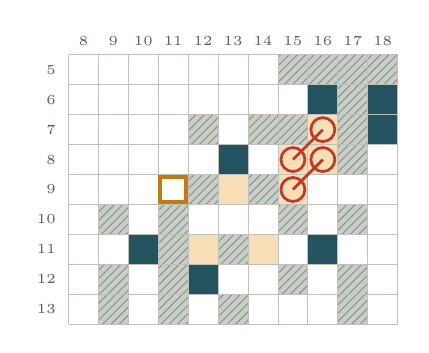
\begin{tikzpicture}[x=0.38cm,y=0.38cm,baseline=(current bounding box.north)]
\node[font=\tiny,text=inksoft] at (0.5,0.45) {8};
\node[font=\tiny,text=inksoft] at (1.5,0.45) {9};
\node[font=\tiny,text=inksoft] at (2.5,0.45) {10};
\node[font=\tiny,text=inksoft] at (3.5,0.45) {11};
\node[font=\tiny,text=inksoft] at (4.5,0.45) {12};
\node[font=\tiny,text=inksoft] at (5.5,0.45) {13};
\node[font=\tiny,text=inksoft] at (6.5,0.45) {14};
\node[font=\tiny,text=inksoft] at (7.5,0.45) {15};
\node[font=\tiny,text=inksoft] at (8.5,0.45) {16};
\node[font=\tiny,text=inksoft] at (9.5,0.45) {17};
\node[font=\tiny,text=inksoft] at (10.5,0.45) {18};
\node[font=\tiny,text=inksoft,anchor=east] at (-0.1,-0.5) {5};
\node[font=\tiny,text=inksoft,anchor=east] at (-0.1,-1.5) {6};
\node[font=\tiny,text=inksoft,anchor=east] at (-0.1,-2.5) {7};
\node[font=\tiny,text=inksoft,anchor=east] at (-0.1,-3.5) {8};
\node[font=\tiny,text=inksoft,anchor=east] at (-0.1,-4.5) {9};
\node[font=\tiny,text=inksoft,anchor=east] at (-0.1,-5.5) {10};
\node[font=\tiny,text=inksoft,anchor=east] at (-0.1,-6.5) {11};
\node[font=\tiny,text=inksoft,anchor=east] at (-0.1,-7.5) {12};
\node[font=\tiny,text=inksoft,anchor=east] at (-0.1,-8.5) {13};
\fill[blockedc] (7,0) rectangle (8,-1);
\fill[pattern=north east lines,pattern color=hatch] (7,0) rectangle (8,-1);
\fill[blockedc] (8,0) rectangle (9,-1);
\fill[pattern=north east lines,pattern color=hatch] (8,0) rectangle (9,-1);
\fill[blockedc] (9,0) rectangle (10,-1);
\fill[pattern=north east lines,pattern color=hatch] (9,0) rectangle (10,-1);
\fill[blockedc] (10,0) rectangle (11,-1);
\fill[pattern=north east lines,pattern color=hatch] (10,0) rectangle (11,-1);
\fill[chosen] (8,-1) rectangle (9,-2);
\fill[blockedc] (9,-1) rectangle (10,-2);
\fill[pattern=north east lines,pattern color=hatch] (9,-1) rectangle (10,-2);
\fill[chosen] (10,-1) rectangle (11,-2);
\fill[blockedc] (4,-2) rectangle (5,-3);
\fill[pattern=north east lines,pattern color=hatch] (4,-2) rectangle (5,-3);
\fill[blockedc] (6,-2) rectangle (7,-3);
\fill[pattern=north east lines,pattern color=hatch] (6,-2) rectangle (7,-3);
\fill[blockedc] (7,-2) rectangle (8,-3);
\fill[pattern=north east lines,pattern color=hatch] (7,-2) rectangle (8,-3);
\fill[candtint] (8,-2) rectangle (9,-3);
\fill[blockedc] (9,-2) rectangle (10,-3);
\fill[pattern=north east lines,pattern color=hatch] (9,-2) rectangle (10,-3);
\fill[chosen] (10,-2) rectangle (11,-3);
\fill[chosen] (5,-3) rectangle (6,-4);
\fill[candtint] (7,-3) rectangle (8,-4);
\fill[candtint] (8,-3) rectangle (9,-4);
\fill[blockedc] (9,-3) rectangle (10,-4);
\fill[pattern=north east lines,pattern color=hatch] (9,-3) rectangle (10,-4);
\fill[blockedc] (4,-4) rectangle (5,-5);
\fill[pattern=north east lines,pattern color=hatch] (4,-4) rectangle (5,-5);
\fill[candtint] (5,-4) rectangle (6,-5);
\fill[blockedc] (6,-4) rectangle (7,-5);
\fill[pattern=north east lines,pattern color=hatch] (6,-4) rectangle (7,-5);
\fill[candtint] (7,-4) rectangle (8,-5);
\fill[blockedc] (1,-5) rectangle (2,-6);
\fill[pattern=north east lines,pattern color=hatch] (1,-5) rectangle (2,-6);
\fill[blockedc] (3,-5) rectangle (4,-6);
\fill[pattern=north east lines,pattern color=hatch] (3,-5) rectangle (4,-6);
\fill[blockedc] (7,-5) rectangle (8,-6);
\fill[pattern=north east lines,pattern color=hatch] (7,-5) rectangle (8,-6);
\fill[blockedc] (9,-5) rectangle (10,-6);
\fill[pattern=north east lines,pattern color=hatch] (9,-5) rectangle (10,-6);
\fill[chosen] (2,-6) rectangle (3,-7);
\fill[blockedc] (3,-6) rectangle (4,-7);
\fill[pattern=north east lines,pattern color=hatch] (3,-6) rectangle (4,-7);
\fill[candtint] (4,-6) rectangle (5,-7);
\fill[blockedc] (5,-6) rectangle (6,-7);
\fill[pattern=north east lines,pattern color=hatch] (5,-6) rectangle (6,-7);
\fill[candtint] (6,-6) rectangle (7,-7);
\fill[chosen] (8,-6) rectangle (9,-7);
\fill[blockedc] (1,-7) rectangle (2,-8);
\fill[pattern=north east lines,pattern color=hatch] (1,-7) rectangle (2,-8);
\fill[blockedc] (3,-7) rectangle (4,-8);
\fill[pattern=north east lines,pattern color=hatch] (3,-7) rectangle (4,-8);
\fill[chosen] (4,-7) rectangle (5,-8);
\fill[blockedc] (7,-7) rectangle (8,-8);
\fill[pattern=north east lines,pattern color=hatch] (7,-7) rectangle (8,-8);
\fill[blockedc] (9,-7) rectangle (10,-8);
\fill[pattern=north east lines,pattern color=hatch] (9,-7) rectangle (10,-8);
\fill[blockedc] (1,-8) rectangle (2,-9);
\fill[pattern=north east lines,pattern color=hatch] (1,-8) rectangle (2,-9);
\fill[blockedc] (3,-8) rectangle (4,-9);
\fill[pattern=north east lines,pattern color=hatch] (3,-8) rectangle (4,-9);
\fill[blockedc] (5,-8) rectangle (6,-9);
\fill[pattern=north east lines,pattern color=hatch] (5,-8) rectangle (6,-9);
\fill[blockedc] (9,-8) rectangle (10,-9);
\fill[pattern=north east lines,pattern color=hatch] (9,-8) rectangle (10,-9);
\draw[gridc,line width=0.3pt,step=1] (0,-9) grid (11,0);
\draw[candc,line width=1.4pt] (3.07,-4.07) rectangle (3.93,-4.93);
\draw[bad,line width=1pt] (8.5,-2.5) -- (7.5,-3.5) (8.5,-2.5) circle (0.4) (7.5,-3.5) circle (0.4);
\draw[bad,line width=1pt] (8.5,-3.5) -- (7.5,-4.5) (8.5,-3.5) circle (0.4) (7.5,-4.5) circle (0.4);
\end{tikzpicture}
\caption{Swept map seed 1, superlattice placement tiles, as one pass reports it. Left: $Z=(9,15)$ forces the seats $(8,15)$ and $(7,16)$, which are diagonal neighbours (red); $(11,15)$ (also outlined) forces $(9,15)$'s cells and runs into the same pair. Right: $(9,11)$ is refuted only through its n-ary facts; its chain up to the first contradiction has 8 cells and two blocking pairs.}
\end{figure}

One pass on this map reports three refuted candidates: $(9,15)$, $(11,15)$ and $(9,11)$. Every chain is taken up to its \emph{first} contradiction only (\code{Base.chain\_until\_contradiction}, and the n-ary step stops there too): whatever would follow from placing two cells that block each other is worthless.

%------------------------------------------------------------------
\section{Why a refutation is permanent}

Forcing is a logical consequence of the current state $S$: ``$Z$ chosen'' together with $S$ implies every cell of $Z$'s chain. More placements only add to $S$: conditions shrink (a chosen member drops out) or die (a blocked member), and nothing derived from $S$ is ever withdrawn. So if $Z$ and $S$ lead to two chosen diagonal neighbours, which is a pixel no cell can cover (F\,4, F\,9), then so do $Z$ and every later state. \textbf{No completion of the map contains $Z$.}

Concretely for $(9,15)$: if $(8,15)$ is later chosen from elsewhere, it blocks $(7,16)$, which $(9,15)$ still forces; if $(7,16)$ gets blocked, $(9,15)$ forces a blocked cell. Either way it is the hole again. The earlier assumption that ``once one of the blocked cells is chosen, $Z$ becomes eligible again'' (12 November) is wrong.

Hence the \textbf{unblocking rule}: a refuted candidate is blocked. In the algebra this is the size-1 defect term $\T{Z}\to\bot$ (F\,9); its effect is the one a chosen diagonal neighbour has: every condition naming $Z$ dies. It stands beside the \textbf{seat rule} (a block with three corners blocked and one free: the free cell is chosen). Both turn a fact that holds in every completion into a state, and both are applied by the CPU between passes.

\paragraph{No freedom is lost.} Blocking $Z$ removes no valid completion, since none contains $Z$. A seat the block creates is chosen in every completion too: with $Z$ out of every completion, the block's last free corner is its only cover. The set of valid completions is the same before and after an unblocking step.

%------------------------------------------------------------------
\section{As implemented: the clean split}

The pass is \emph{analysis only}: it answers ``if $Z$ is chosen, this will happen'' and never changes a cell's \code{.state}. Acting on its findings is the CPU's placement step.

\begin{algebra}\raggedright
\textbf{Pass} (\code{Pyramid.onepass}), on a fixed state:\\
\quad 1.\ \code{init\_map}: conditions from \code{.state}\\
\quad 2.\ refuted from single links $\Rightarrow$ suspended (\code{Base.suspend\_contradictory})\\
\quad 3.\ up and down passes with round trips; the n-ary step stops a candidate at its first contradiction\\
\quad 4.\ refuted from n-ary facts (\code{mem.nary\_contradictory}, \code{Base.contradictory\_after\_nary})\\
\qquad $\Rightarrow$ suspended from the start, pass rerun from 1\\
\quad 5.\ report: \code{mem.refuted} $=\{Z: (\text{chain},\ \text{blocking pairs})\}$\\[0.4em]
\textbf{CPU placement step} (\code{Pyramid.unblock}):\\
\quad 6.\ unblocking rule: every reported $Z$ gets \code{.state = blocked}\\
\quad 7.\ seat rule: fill seats to a fixed point (\code{Pyramid.fill\_seats}); a real block\\
\qquad with four blocked corners raises \code{Uncompletable}\\
\quad 8.\ log the round in \code{mem.unblock\_rounds}; next pass\\[0.4em]
\cmt{\code{Pyramid.analyse\_and\_unblock} alternates the two until a pass refutes nothing.}
\end{algebra}

Within the pass a refuted candidate is merely \emph{suspended}: it is no candidate, starts no chain, and its own \code{.blocked} entry is $(Z,Z)$. Its \code{.state} stays free. Suspension is now only the pass's way of not using what it has just shown impossible; it is lifted by the CPU step, which blocks $Z$ for good.

The next \code{init\_map} needs nothing new: a blocked cell with no chosen cell behind it is already handled (\code{Base.blocked\_corner\_conditions}): conditions naming $Z$ are dropped, and the blocks with $Z$ as a corner get conditions for their remaining open corners.

\begin{figure}[H]\centering
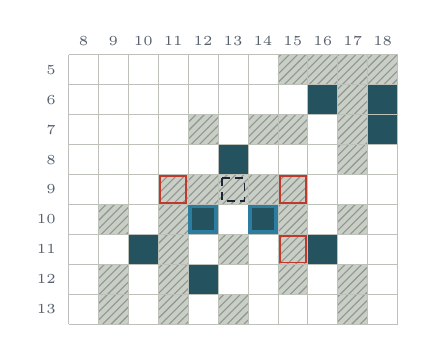
\begin{tikzpicture}[x=0.38cm,y=0.38cm,baseline=(current bounding box.north)]
\node[font=\tiny,text=inksoft] at (0.5,0.45) {8};
\node[font=\tiny,text=inksoft] at (1.5,0.45) {9};
\node[font=\tiny,text=inksoft] at (2.5,0.45) {10};
\node[font=\tiny,text=inksoft] at (3.5,0.45) {11};
\node[font=\tiny,text=inksoft] at (4.5,0.45) {12};
\node[font=\tiny,text=inksoft] at (5.5,0.45) {13};
\node[font=\tiny,text=inksoft] at (6.5,0.45) {14};
\node[font=\tiny,text=inksoft] at (7.5,0.45) {15};
\node[font=\tiny,text=inksoft] at (8.5,0.45) {16};
\node[font=\tiny,text=inksoft] at (9.5,0.45) {17};
\node[font=\tiny,text=inksoft] at (10.5,0.45) {18};
\node[font=\tiny,text=inksoft,anchor=east] at (-0.1,-0.5) {5};
\node[font=\tiny,text=inksoft,anchor=east] at (-0.1,-1.5) {6};
\node[font=\tiny,text=inksoft,anchor=east] at (-0.1,-2.5) {7};
\node[font=\tiny,text=inksoft,anchor=east] at (-0.1,-3.5) {8};
\node[font=\tiny,text=inksoft,anchor=east] at (-0.1,-4.5) {9};
\node[font=\tiny,text=inksoft,anchor=east] at (-0.1,-5.5) {10};
\node[font=\tiny,text=inksoft,anchor=east] at (-0.1,-6.5) {11};
\node[font=\tiny,text=inksoft,anchor=east] at (-0.1,-7.5) {12};
\node[font=\tiny,text=inksoft,anchor=east] at (-0.1,-8.5) {13};
\fill[blockedc] (7,0) rectangle (8,-1);
\fill[pattern=north east lines,pattern color=hatch] (7,0) rectangle (8,-1);
\fill[blockedc] (8,0) rectangle (9,-1);
\fill[pattern=north east lines,pattern color=hatch] (8,0) rectangle (9,-1);
\fill[blockedc] (9,0) rectangle (10,-1);
\fill[pattern=north east lines,pattern color=hatch] (9,0) rectangle (10,-1);
\fill[blockedc] (10,0) rectangle (11,-1);
\fill[pattern=north east lines,pattern color=hatch] (10,0) rectangle (11,-1);
\fill[chosen] (8,-1) rectangle (9,-2);
\fill[blockedc] (9,-1) rectangle (10,-2);
\fill[pattern=north east lines,pattern color=hatch] (9,-1) rectangle (10,-2);
\fill[chosen] (10,-1) rectangle (11,-2);
\fill[blockedc] (4,-2) rectangle (5,-3);
\fill[pattern=north east lines,pattern color=hatch] (4,-2) rectangle (5,-3);
\fill[blockedc] (6,-2) rectangle (7,-3);
\fill[pattern=north east lines,pattern color=hatch] (6,-2) rectangle (7,-3);
\fill[blockedc] (7,-2) rectangle (8,-3);
\fill[pattern=north east lines,pattern color=hatch] (7,-2) rectangle (8,-3);
\fill[blockedc] (9,-2) rectangle (10,-3);
\fill[pattern=north east lines,pattern color=hatch] (9,-2) rectangle (10,-3);
\fill[chosen] (10,-2) rectangle (11,-3);
\fill[chosen] (5,-3) rectangle (6,-4);
\fill[blockedc] (9,-3) rectangle (10,-4);
\fill[pattern=north east lines,pattern color=hatch] (9,-3) rectangle (10,-4);
\fill[blockedc] (3,-4) rectangle (4,-5);
\fill[pattern=north east lines,pattern color=hatch] (3,-4) rectangle (4,-5);
\fill[blockedc] (4,-4) rectangle (5,-5);
\fill[pattern=north east lines,pattern color=hatch] (4,-4) rectangle (5,-5);
\fill[blockedc] (5,-4) rectangle (6,-5);
\fill[pattern=north east lines,pattern color=hatch] (5,-4) rectangle (6,-5);
\fill[blockedc] (6,-4) rectangle (7,-5);
\fill[pattern=north east lines,pattern color=hatch] (6,-4) rectangle (7,-5);
\fill[blockedc] (7,-4) rectangle (8,-5);
\fill[pattern=north east lines,pattern color=hatch] (7,-4) rectangle (8,-5);
\fill[blockedc] (1,-5) rectangle (2,-6);
\fill[pattern=north east lines,pattern color=hatch] (1,-5) rectangle (2,-6);
\fill[blockedc] (3,-5) rectangle (4,-6);
\fill[pattern=north east lines,pattern color=hatch] (3,-5) rectangle (4,-6);
\fill[chosen] (4,-5) rectangle (5,-6);
\fill[chosen] (6,-5) rectangle (7,-6);
\fill[blockedc] (7,-5) rectangle (8,-6);
\fill[pattern=north east lines,pattern color=hatch] (7,-5) rectangle (8,-6);
\fill[blockedc] (9,-5) rectangle (10,-6);
\fill[pattern=north east lines,pattern color=hatch] (9,-5) rectangle (10,-6);
\fill[chosen] (2,-6) rectangle (3,-7);
\fill[blockedc] (3,-6) rectangle (4,-7);
\fill[pattern=north east lines,pattern color=hatch] (3,-6) rectangle (4,-7);
\fill[blockedc] (5,-6) rectangle (6,-7);
\fill[pattern=north east lines,pattern color=hatch] (5,-6) rectangle (6,-7);
\fill[blockedc] (7,-6) rectangle (8,-7);
\fill[pattern=north east lines,pattern color=hatch] (7,-6) rectangle (8,-7);
\fill[chosen] (8,-6) rectangle (9,-7);
\fill[blockedc] (1,-7) rectangle (2,-8);
\fill[pattern=north east lines,pattern color=hatch] (1,-7) rectangle (2,-8);
\fill[blockedc] (3,-7) rectangle (4,-8);
\fill[pattern=north east lines,pattern color=hatch] (3,-7) rectangle (4,-8);
\fill[chosen] (4,-7) rectangle (5,-8);
\fill[blockedc] (7,-7) rectangle (8,-8);
\fill[pattern=north east lines,pattern color=hatch] (7,-7) rectangle (8,-8);
\fill[blockedc] (9,-7) rectangle (10,-8);
\fill[pattern=north east lines,pattern color=hatch] (9,-7) rectangle (10,-8);
\fill[blockedc] (1,-8) rectangle (2,-9);
\fill[pattern=north east lines,pattern color=hatch] (1,-8) rectangle (2,-9);
\fill[blockedc] (3,-8) rectangle (4,-9);
\fill[pattern=north east lines,pattern color=hatch] (3,-8) rectangle (4,-9);
\fill[blockedc] (5,-8) rectangle (6,-9);
\fill[pattern=north east lines,pattern color=hatch] (5,-8) rectangle (6,-9);
\fill[blockedc] (9,-8) rectangle (10,-9);
\fill[pattern=north east lines,pattern color=hatch] (9,-8) rectangle (10,-9);
\draw[gridc,line width=0.3pt,step=1] (0,-9) grid (11,0);
\draw[bad,line width=0.7pt] (3.06,-4.06) rectangle (3.94,-4.9399999999999995);
\draw[ink,densely dashed,line width=0.6pt] (5.12,-4.12) rectangle (5.88,-4.88);
\draw[bad,line width=0.7pt] (7.06,-4.06) rectangle (7.9399999999999995,-4.9399999999999995);
\draw[bad,line width=0.7pt] (7.06,-6.06) rectangle (7.9399999999999995,-6.9399999999999995);
\draw[focus,line width=1.4pt] (4.07,-5.07) rectangle (4.93,-5.93);
\draw[focus,line width=1.4pt] (6.07,-5.07) rectangle (6.93,-5.93);
\end{tikzpicture}
\caption{After the CPU's unblocking step. Red outline: the three refuted candidates, now blocked. Blue outline: the seats this creates, $(10,12)$ and $(10,14)$, now chosen. Dashed: the cells those seats block. The next pass on this state refutes nothing.}
\end{figure}

\paragraph{Results.}
\begin{center}\small
\begin{tabular}{@{}p{0.27\linewidth}p{0.07\linewidth}p{0.3\linewidth}p{0.28\linewidth}@{}}
\toprule
map & round & blocked & seats filled\\
\midrule
swept seed 1, superlattice & 1 & $(9,11)$, $(9,15)$, $(11,15)$ & $(10,12)$, $(10,14)$\\
swept seed 2, superlattice & 1 & $(10,11)$, $(11,3)$, $(16,15)$, $(16,17)$, $(17,11)$ & $(17,14)$, $(17,16)$, $(18,12)$, $(18,16)$\\
 & 2 & $(15,11)$ & --\\
swept seed 2, \code{build\_swept\_map} layout & 1 & $(16,15)$, $(16,17)$ & $(17,14)$, $(17,16)$, $(18,12)$, $(18,16)$\\
frozen area & -- & -- & --\\
\bottomrule
\end{tabular}
\end{center}
On seed 2 with superlattice tiles, $(15,11)$ is refuted only on the state the first round leaves: a refutation that needs the blocks and seats of an earlier round.

%------------------------------------------------------------------
\section{Approach 1: suspending (12 to 15 November)}

The refuted candidate was suspended for the pass and nothing else happened. The state stayed as it was, so every later pass found the same refutation again and suspended $Z$ again. The idea behind it was a ``harmless postponement'': once one of the blocking cells is chosen by another placement, $Z$ would become eligible again. Section 2 shows that this never happens.

\begin{itemize}[leftmargin=*,itemsep=0.2em]
\item \textbf{Sound, but it keeps information out.} No pass ever learns that $Z$ is impossible as a fact of the map: the conditions naming $Z$ stay alive, the blocks with $Z$ as a corner never get their conditions, and the seats that blocking $Z$ makes, $(10,12)$ and $(10,14)$ here, are never found to be forced.
\item \textbf{Repeated work.} The refutation is derived anew in every pass, including the n-ary ones like $(9,11)$, which cost a rerun of the whole pass each time.
\item \textbf{Same completions.} Nothing invalid is ever chosen, since a suspended $Z$ is never a decision; but the map does not converge to a state where the analysis finds nothing left to refute.
\end{itemize}

%------------------------------------------------------------------
\section{Approach 2: unblocking inside the pass (15 to 16 November)}

The first implementation applied the unblocking rule \emph{inside} \code{onepass}: a refuted candidate was blocked at once, the seats that made were filled, and the pass restarted from \code{init\_map} on the new state, until a pass refuted nothing.

\begin{itemize}[leftmargin=*,itemsep=0.2em]
\item \textbf{The analysis placed cells.} Filling $(10,14)$ is a placement, made in a step meant to answer ``if $Z$ is chosen, this will happen''. Forced or not, the analysis then reported results for a state the caller had not handed it. On the GPU this would mean the device writing \code{.state}, which the design leaves to the CPU.
\item \textbf{Failure in the wrong place.} On the raw swept map with seed 0, whose open seats cannot all be filled, the analysis itself raised \code{Uncompletable}, because it filled those seats. A map problem surfaced as an analysis failure.
\item \textbf{More information within a call, in smaller steps.} Each refutation found before the up pass was blocked before the rest was analysed. On seed 1, $(9,15)$ and $(11,15)$ were blocked first; on that state $(9,11)$ was refuted by its single links alone (pair $(10,13)/(11,12)$), one round later. That needed two rounds where the clean split needs one.
\item \textbf{Checking got harder.} A refutation found in a later round could rest on an earlier round's blocks, so every check had to replay each round on its own state.
\end{itemize}

%------------------------------------------------------------------
\section{Side by side}

\begin{center}\small
\begin{tabular}{@{}p{0.23\linewidth}p{0.22\linewidth}p{0.22\linewidth}p{0.22\linewidth}@{}}
\toprule
 & suspending & unblocking in the pass & clean split (implemented)\\
\midrule
refuted $Z$ & no candidate for the pass & blocked at once & no candidate for the pass; reported\\
\code{.state} changed by the pass & no & yes: blocks and seats & no\\
who blocks $Z$ & nobody & the pass & the CPU's placement step\\
seats after blocking & never filled & filled by the pass & filled by the CPU step\\
refutation found again & every pass & no & no\\
same valid completions & yes & yes & yes\\
learns from the blocks & never & within the same call & from the next pass on\\
seed 1 & 3 suspended each pass & 2 rounds & 1 round\\
\code{.blocked} after the pass & pairs and $(Z,Z)$ & pairs only & pairs and $(Z,Z)$\\
\code{Uncompletable} raised in & nowhere & the analysis & the CPU step\\
\bottomrule
\end{tabular}
\end{center}

%------------------------------------------------------------------
\section{Open points}
\begin{enumerate}[leftmargin=*,itemsep=0.3em]
\item \textbf{Blocking pairs are not unblocked.} Two candidates from different placement tiles that block each other, like $(3,5)$ and $(5,9)$ on seed 1, are each possible alone; only the pair is excluded. They stay in \code{.blocked} and constrain the decisions, not the state.
\item \textbf{Cost of the split.} What a block teaches is used one pass later. Since the CPU step is cheap and the next pass is needed anyway after the decisions, this is expected to cost little; it has not been measured.
\item \textbf{The decisions.} \code{analyse\_and\_unblock} has no decisions yet. In the full CPU main, the unblocking and seat rules go into the same placement step as the chosen candidates, and the order within that step needs fixing: block refuted candidates before or after placing the decisions, which may refute more.
\end{enumerate}

\end{document}
